\begin{abstract}
    Ce document est rédigé dans le cadre de la première anné d'alternance de Lucas Sovre au sein de \acrshort{edf} R\&D, en partenariat avec l'école ESIEE-IT.
    Mon tuteur entreprise est un ingénieur chercheur : julien Caron. Bien que ce rapport ne présente pas de données confidentielles, sa diffusion dois rester réduite.
\end{abstract}
\chapter{Présentation de EDF.}
\section{L'histoire de EDF.}
Dans  les  années  30,  deux  cent  entreprises privées  assurent  la  production,  une  centaine le  transport  et  plus  de  mille  la  distribution  de l’électricité. L’approvisionnement et les tarifs de l’électricité  sont  alors  très  différents  selon les prestataires et les régions.Après-guerre, la création d’un service public unique  de  l’électricité  devient  alors  une nécessité.  La  première  tâche  du  groupe  \acrshort{edf} est  de  reconstruire  entièrement  le  réseau  de transport   partiellement   détruit   pendant   la guerre   et   de   relancer   la   construction   de grands   ouvrages   hydrauliques   dont   certain avait été  interrompu  par  la  guerre. De  1946  à 1970, la France achète à l’étranger 76\% de son approvisionnement  en  énergie  et  le  pétrole constitue 84\% de ses importations.Dès  1973,  à  la  suite  de  la  crise  pétrolière,  la France se tourne vers la production D’électricité à    partird’énergie nucléaire  et  annonce  la  construction  des  13 premières  centrales  entre  1974  et  1975,  avec une   volonté   :   garantir   son   indépendance énergétique.

Avec  les  années,  \acrshort{edf}  acquiert,  une  expertise, un savoir-faire technologique et des compétences  de  haut  niveau,  et  s’impose  comme un leader mondial dans le domaine de l’énergie.

A   la   fin   du   siècle   dernier, le   marché   de l’électricité s’ouvre à la concurrence et \acrshort{edf} se développe en Europe et à l’international. Les échanges s’intensifient, ainsi que la prise en compte des problématiques de développement durable. \acrshort{edf} lance le chantier d’une  centrale  nucléaire  de nouvelle génération  à  Flamanville.  La  construction  de ce premier EPR en France (réacteur pressurisé européen)  est  une  étape  essentielle  dans  la préparation du  Renouvellement du parc nucléaire d’\acrshort{edf}.

\section{Fonctionnement d'une centrale nucléaire.}

Une centrale nucléaire REP (Réacteur à Eau Préssurisée) repose sur la fission nucléaire afin de transformer de l’énergie nucléaire en énergie électrique. On trouve dans le cœur du réacteur nucléaire le matériau fissible, dans notre cas il s’agit de l’uranium 235,  on  va  déclencher  dans  celui-ci une réaction en chaine de façons à produire de l’énergie thermique et ainsi chauffer l’eau du circuit primaire circulant dans la cuve du réacteur. Elle est à 325c   mais   reste   liquide   grâce   au   pressuriseur   qui   maintient   le   circuit   primaire   à   155   BarL’eau sortant de la cuve va passer dans le faisceau tubulaire de chaque générateur de vapeur afin de pouvoir léguer son énergie thermique à l’eau du circuit secondaire. Celle-ci en circulant  dans les GV va se transformer en vapeur pour alimenter le groupe turbo alternateur comprenant une turbine et un alternateur.

La  turbine  est  constituée  d'un  corps  haute  pression  (HP)  et  de  plusieurs  corps  basse  pression  (BP), après passage dans le corps HP, la  vapeur passe ensuite dans les générateurs sécheurs surchauffeurs (GSS) afin d’améliorer son titre avant d'alimenter les corps BP.Les turbines BP et la turbine HP se trouvent sur le même arbre donc elles tournent à la même vitesse et entraînent un alternateur qui produit l'électricitéLa  vapeur  est  ensuite  condensée  en  eau  puis  envoyée  vers  les  GV  au  travers  du  poste  d'eau  qui permet d'améliorer le rendement de l'installation.Le condenseur lui va être refroidi par un troisième circuit lié au fleuve passant près de la centrale ou par des aéroréfrigérants.

Il  est  important  de  noter  que  les  fluides  des  circuits  primaire,  secondaire  et  tertiaire  échangent  de l’énergie entre eux mais ne sont en aucun cas en contact.Ces trois circuit sont strictement indépendant les uns des autres
\centering{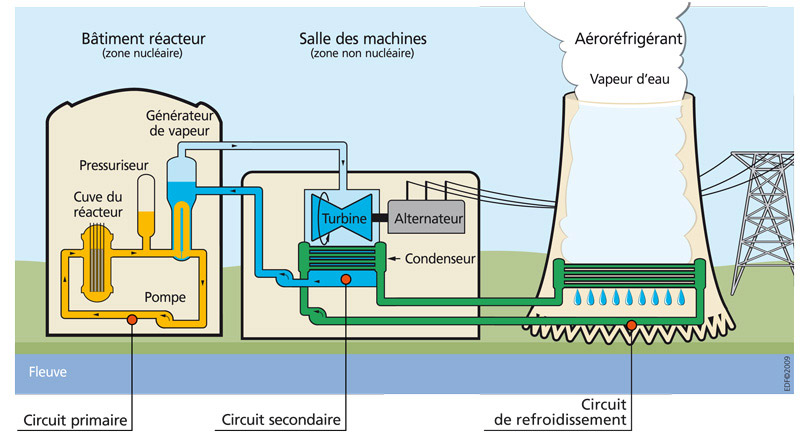
\includegraphics[scale=0.5]{images/schemaREP.jpg}}
~\cite[IRSN]{IRSN_rep_schema}

\justify
\section{La recherche et développement}

\subsection{Présentation de la R\&D}

La R\&D est au cœur d’enjeux majeurs du Groupe \acrshort{edf}. Elle couvre l’ensemble des métiers et activités du secteur de l’énergie. Elle appuie au quotidien les métiers et les filiales en cohérence avec le projet du Groupe \acrshort{edf}, Cap 2030. Deux missions animent les chercheurs : améliorer la performance dans toutes les activités d’aujourd’hui et préparer l’avenir en travaillant sur les technologies de rupture.

En quelques chiffres \acrshort{edf} R\&D c'est 518 Millions d'euro de budget, 160 doctorants (en 2020), 1800 salariés et 11 petaflops de capacité de calcul.

\subsection{Mon environement de travail au sein de la R\&D}
Je travaille sur le site de \acrshort{edf} lab Paris-saclay qui est situé au coeur du plateau universitaire de saclay. Ses activités et domaines de recherche sont trés diversifiés : mécanique vibratoire, génie logiciel, mathématiques et simulation numérique, économie de l'électricité, management des risques industriels, NTIC et architectures de comptage et digitales, traitement des méga-données, relation client et création de nouveaux services...

Je travaille au sein du département Pericles, dans le groupe I2A. Il est spécialisé dans l'architécture informatique.

\textit{
    "En informatique, architecture désigne la structure générale inhérente à un système informatique, l'organisation des différents éléments du système (logiciels et/ou matériels et/ou humains et/ou informations) et des relations entre les éléments. Cette structure fait suite à un ensemble de décisions stratégiques prises durant la conception de tout ou partie du système informatique, par l'exercice d'une discipline technique et industrielle du secteur de l'informatique dénommée elle aussi architecture, et dont le responsable est l'architecte informatique."
}   \cite{wikipedia_archi_info}

Mes collégues sont éssentiellement des ingénieurs chercheurs et mon travail consiste à participer aux projets de façons active pendant toutes les phases : 
\begin{itemize}
\item Caractérisation des besoins.
\item Prototypage d'une "\gls{POC}".
\item Décision des choix architecturaux.
\item Developpement de la solution.
\item Prise en compte du retour client.
\end{itemize}

\chapter{Mes projets.}
\section{Projet ARDEN}
\subsection{Contexte}
Les centrales nucléaires francaises s'appuient sur de multiples systèmes de sécutiés pour garantire une exploitation en toute suretée. L'un des principaux éléments de ce système est l'enceinte du réacteur nucléaire, plus comunément appelé \acrshort{br} (Batiment Réacteur).

\textit{"Le bâtiment réacteur (ou enceinte de confinement) [...] assure le confinement des substances radioactives par rapport à l’environnement extérieur et la protection du réacteur contre les agressions externes.  
Le bâtiment réacteur abrite la cuve, le circuit primaire, une partie des circuits secondaires [...]
De manière schématique, le bâtiment du réacteur est constitué d’un cylindre en béton surmonté d’un dôme en béton (toît du bâtiment) qui forme une enveloppe résistante et à étanchéité spécifiée.
[...]Elle est conçue pour résister à la pression atteinte lors des accidents retenus à la conception du réacteur (4 à 5 bars absolus) et pour rester étanche dans ces circonstances. Les parois en béton reposent sur un radier lui-même en béton qui constitue le socle du bâtiment."}  \cite[IRSN]{IRSN_suretee}

Les exploitants de tout \acrshort{cnpe} mène réguliérement des essais afin d'assurer une disponibilitée maximum de ses organes de suretées. 

Dans ce cadre, lors de chaque \gls{VD} des éssais sont menés sur le \acrshort{br}. Notament une épreuve d'étanchéité aucours de laquelle le \gls{br} est monté en pression à 5bar , soit environt 5 fois la pression atmosphérique (1 atm = 1.013bar).

Les essais menés sont alors source de nombreuse données éssentielles.

La R\&D de \gls{edf} à décidé de mener des recherches pouvant prédire le comportement du viellisement des reacteurs nucléaires. Pour cela une réplique éxacte à l'échelle 1/3 à été crée. Grâce à divers procédés physico-chimiques celle ci vielli neuf fois plus vite que les batiments réacteurs nucléaire du parc francais. Ainsi en reproduisant le cycle de vie des vrais \gls{cnpe} sur ce \gls{br}. Les données générées lors des \gls{VD} sur cette réplique nous permettent de prédire précisément l'évolution des \gls{br} en production.

Lors de ces experimentations la grande quantitée de données générées nécéssitent un système d'informations robuste et perrin.
\subsubsection{Caractérisation du besoin.}

Par analogie avec le Carnet de Santé, le système ARDEN a pour objectif d’être le référentiel des informations connues   sur   les   enceinte,   organisées dans   le   temps   par   la   séquence   des   évènements   majeurs (construction, mise en service, visites de contrôle, travaux d’inspection, travaux de réparation), puis dans l’espace au moyen d’une partition géométrique du bâtiment en Zones Fonctionnelles.

La  modélisation  scientifique  et  la simulation  numérique  peuvent  alors  venir  aider  le  médecin  à  mieux comprendre les mécanismes à l’œuvre (séchage et fluage qui déterminent la dégradation de l’enceinte), puis dans une certaine mesure prévoir l’évolution et proposer des remédiations (prédiction  de  fuite  et analyse des scénarios de recouvrement des compléments d’étanchéité).

\centering{
    \fbox{
        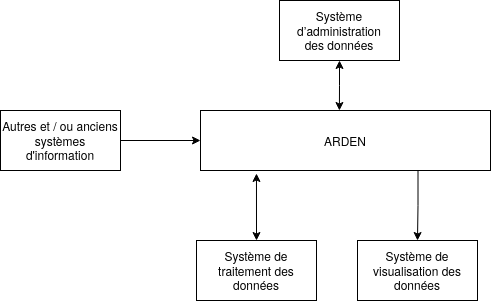
\includegraphics[scale=0.5]{images/ARDEN_generalNeed.png}
    }
}

\justify
\subsection{Choix d'architécture informatique.}

\subsubsection{Choix de l'interface d'accés au système.}

Le système ARDEN sera accèssible sous forme d'\gls{api} \gls{rest}. Ce choix est motivé par le fait que l' API RESTful est un standard de l'industrie premetants de facilement déployer le système sous forme d'architécture microServices. De plus la forme standard des \gls{api} \gls{rest} facilite grandement les intégrations avec d'autres systèmes.

\begin{minipage}{0.90\textwidth}
    \underline{
        Les \gls{api} \gls{rest} :
    }
    L'architecture REST a été créée par l'informaticien Roy Fielding en 2000 dans sathèse de doctorat Architectural Styles and the Design of Network-basedSoftwareArchitectures . \cite{REST_theses}
    Dans le cas d'une \gls{api} web RESTful des standard suplémentaires sont appliqués :
    \begin{itemize}
        \item Architécture serveur-client.
        \item Sans état. (L’API traite chaque requête comme une première demande.)
        \item Mise en cache. (Les données fréquement demandées sont mises en cache pour réduire la bande passante.)
        \item Interface uniforme. (Méthodes de communication post, get, put, delete)
        \item Possibilitée de plusieurs couches.
    \end{itemize}
    Comunément une interface \gls{api} \gls{rest} web implémente au minimum les 4méthodes html par point d'accés (GET, POST, PUT, DELETE). Une cinquième méthode(PATCH) existe mais est parfois confondue avec PUT dans son utilisation. Leurdifférences est que PATCH permet de mettre à jour uniquement certains champs d'unobjects. Alors que PUT remplace complétement un object défini par celui envoyé.
\end{minipage}

\centering{
    \fbox{
    \begin{minipage}{0.90\textwidth}
    \underline{Note :}

    Dans certains cas ne pas donner accés à certaines méthodes HTTP pour certains endpoint peut être un choix délibéré d'architecture afin de limiter les actions d'utilisateurs. 

    \underline{Exemple :} Donner uniquement accés à la visualisation des données à certains utilisateurs.
    \end{minipage}
    }
}

\justify
\subsubsection{Choix de la technologie de sauvegarde des données.}

La sauvegarde des données dois être realisée dans une \gls{bdd} car cette technologie permet de centraliser, sécuriser et sipmlifier les transaction de données.

Il existe dans l'industrie actuelle deux standard principaux en terme de \gls{bdd} :
\begin{itemize}
    \item \gls{bdd} relationelle (SQL ou SGBDR) : Système qui est basée sur un architécture en tables de données.
    \item \gls{bdd} non relationelle (noSQL) : Système qui n'as pas d'architecture prédéfinie, qui est basée sur un système de clé-valeur pour lier les objects entre eux. \cite{BDD_theses}
\end{itemize}

Dans le cas du projet ARDEN, le retour d'experience de cette technologie, les avantages d'évotulivité et de disponibilitée face à de grands nombres de transaction ont portés notre choix sur une \gls{bdd} relationelle.

Dans les bases de données relationelle de multiples moteurs de \gls{bdd} existent (Postgresql, MySql, Sqlite3 , Oracle Database ...)

Le choix de moteur de \gls{bdd} dois être mené en prenant en compte les propriétées \gls{acid} :
\begin{itemize}
    \item Atomicité : Cela assure qu'une transaction soit effectué de facons totale ou aucunement (si une requête de 500 ligne est performée, mais que une seule ligne pose problème : la totalité de la transaction est abandonnée). 
    \item Cohérence : Toutes les requêtes doivent strictement respecter les règles de la base de donnée pour être performmées.
    \item Isolation : Chaque transaction doit s'exécuter en isolation totale : si T1 et T2 s'exécutent simultanément, alors chacune doit demeurer indépendante de l'autre. 
    \item durabilité : Assure que les données restes intégres dans le temps, sans être altérées par des facteurs extérieurs.
    \cite{wikipedia_acid}
\end{itemize}

Il faut noter que ces propriétées ne sont pas toujours désirées. Selon le besoin l'atomicité peut ne pas être voulue lorsque les requêtes ne sont pas reproductibles et que les données sont cruciale.

Dans notre cas nous avons choisi Postgresql pour le retour d'experience positif, sa grande évolutivité et sa polyvalence en terme d'\gls{acid}.

\subsubsection{Choix de technologie de langage logiciel.}

Concernant le language informatique danslequel creer le coeur de l'application ARDEN l'orde des prossibles étant assez vaste (nodejs, python, java, C++, .NET, Golang ...). Notre choix s'est ortienté grace au retour d'experience (pas de technologies émergentes), de la portabilitée du language (execution indépendante du système d'exploitation.), de sa communautée et de son évolutivitée.

Le java répond à toutes ces spécification : 
Le \gls{jdk} permet d'assurer une portabilitée totale du java. Même si il à beacoup evolué depuis, il date de 1995 et possède une des plus grandes communautée de la sphère informatique. Dernièrement, le java est trés évolutif. 

Nous avons également fait le choix d'utiliser SpringBoot : Il s'agit d'un framework java facilitant le development de logiciels profesisonels ortienté web.
Nous avons également décider d'utiliser Gradle pour faciliter la compilation, le dépoiement et la gestion des dépendances de notre projet.

Concernant l'injection de scripts SQL au démarage et la migartion de bases de données : Nous avons choisi d'utiliser Flyway, qui est un outil open-source sans dépendances et sans format ou langage propriétaire.

Nous allons également utiliser un client python sous la forme de paquet pour permettre aux utilisateurs finaux d'appeler l'api de facons simple et sans mauvaises utilisation de la base de donnée.

Le schéma ci-dessous résume l'architécture de ce projet (également disponible en annexe 1) : 

\centering{
    \fbox{
        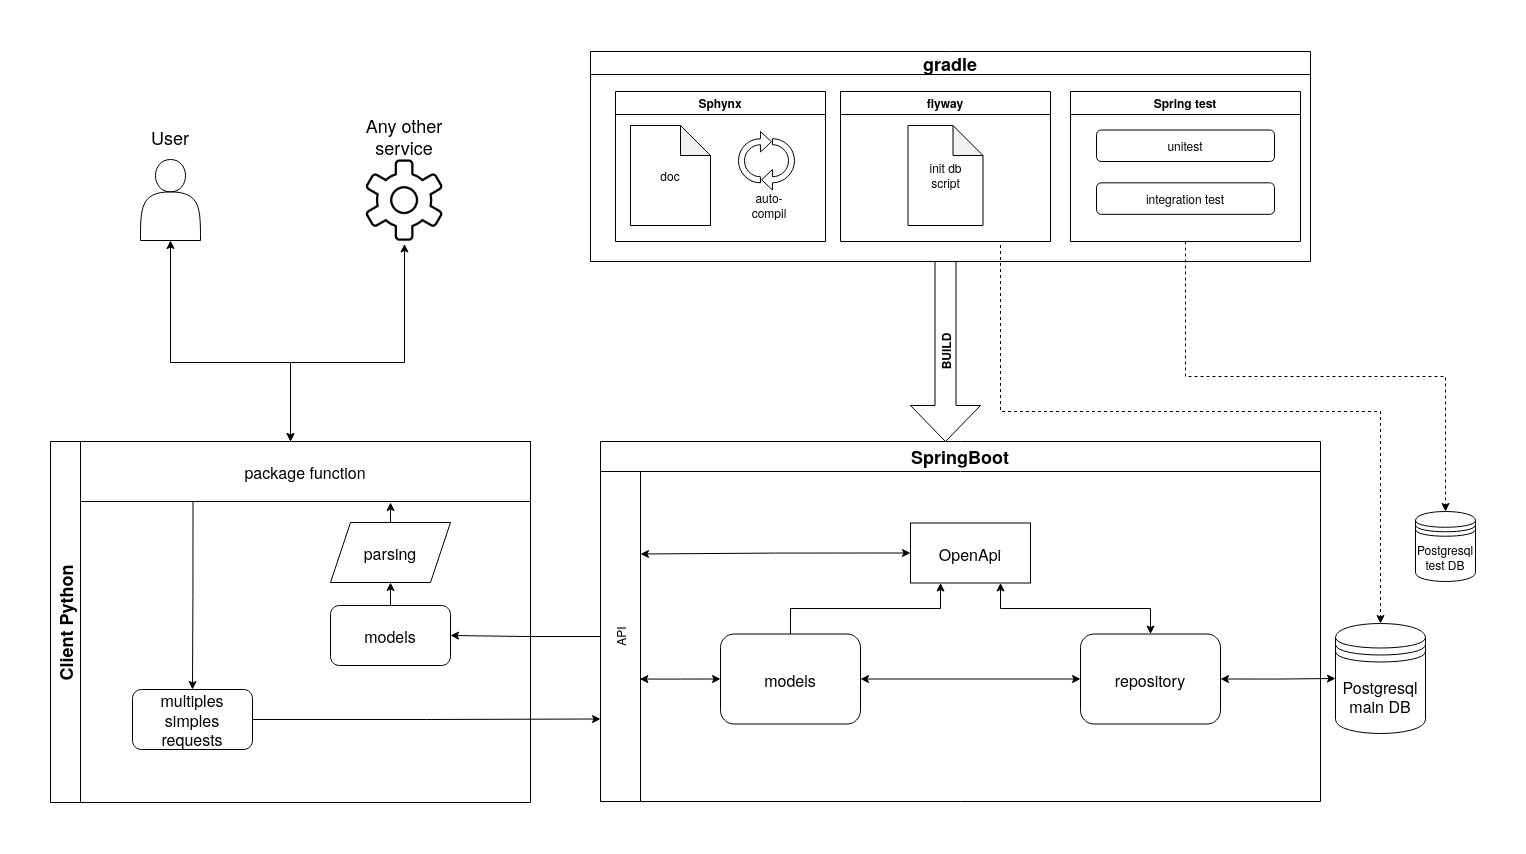
\includegraphics[scale=0.20]{images/ARDEN_techno.png}
    }
}